% v2-acmtog-sample.tex, dated March 7 2012
% This is a sample file for ACM Transactions on Graphics
%
% Compilation using 'acmtog.cls' - version 1.2 (March 2012), Aptara Inc.
% (c) 2010 Association for Computing Machinery (ACM)
%
% Questions/Suggestions/Feedback should be addressed to => "acmtexsupport@aptaracorp.com".
% Users can also go through the FAQs available on the journal's submission webpage.
%
% Steps to compile: latex, bibtex, latex latex
%
% For tracking purposes => this is v1.2 - March 2012
\documentclass{acmtog} % V1.2

%\acmVolume{VV}
%\acmNumber{N}
%\acmYear{YYYY}
%\acmMonth{Month}
%\acmArticleNum{XXX}
%\acmdoi{10.1145/XXXXXXX.YYYYYYY}

\acmVolume{28}
\acmNumber{4}
\acmYear{2019}
\acmMonth{January}
\acmArticleNum{106}
\acmdoi{10.1145/1559755.1559763}

\begin{document}

\markboth{V. F. Pamplona et al.}{Photorealistic Models for Pupil Light Reflex and Iridal Pattern Deformation}

\title{New Routing Algorithm in NoC} % title

\author{KAIFAN CAI {\upshape and} YUJIE HAN
\affil{Shanghai Jiao Tong University}
% NOTE! Affiliations placed here should be for the institution where the
%       BULK of the research was done. If the author has gone to a new
%       institution, before publication, the (above) affiliation should NOT be changed.
%       The authors 'current' address may be given in the "Author's addresses:" block (below).
%       So for example, Mr. Fogarty, the bulk of the research was done at UIUC, and he is
%       currently affiliated with NASA.
}

\maketitle
\begin{abstract}
Network on chips(NoC) is one of the communication systems in SoC(system on chip). And Routing algorithms determine the paths that a packet should take during its journey from the source to the destination. There are several challenges that may appear with routing algorithms such as deadlock, livelock and starvation. Our group would like to design a routing algorithm to decrease the overall latency of transferring the packets.
\end{abstract}

\section{Introduction}
\label{sec:introduction}

Network on chips(NoC) is one of the communication systems in SoC(system on chip). And Routing algorithms determine the paths that a packet should take during its journey from the source to the destination. There are several challenges that may appear with routing algorithms such as deadlock, livelock and starvation. Our group would like to design a routing algorithm to decrease the overall latency of transferring the packets.

After we explored some traditional routing algorithm, we found that there is no routing algorithm choosing the path to transfer the packets referring to the crowdedness of the whole network. But the crowdedness of network will directly influence the efficiency of NoC. So our group are going to design some routing algorithms which will take the crowdedness of the whole network into consideration.

Besides, we will do some experiment to simulate the NoC, in order to estimate the efficiency of our routing algorithm. We also need to compare the results of our routing algorithms with the results of some traditional routing algorithms.
\section{Background}
\label{sec:background}

Let's learn something about NoC and routing algorithm.

NoC is an interconnection network system which enables a decrease in the communication complexity and improve the performance in multi-core SoCs. NoC has three main components i.e., Router, Network Interface and Link as shown in the Fig.1. The Communication between the IP cores is done using routers that are distributed across the whole network and serve as the communication backbone of the NoC. The main purpose of the router in an NoC is to route the packet towards its destination either directly or through other routers. Routing packets in NoC depends on the routing algorithm used, which decides the approach and paths of packets moving through the network. NoC provides high-scalability, less resource under utilization, less complexity and high-performance compared to other communication techniques. [1]

\begin{figure}[h]
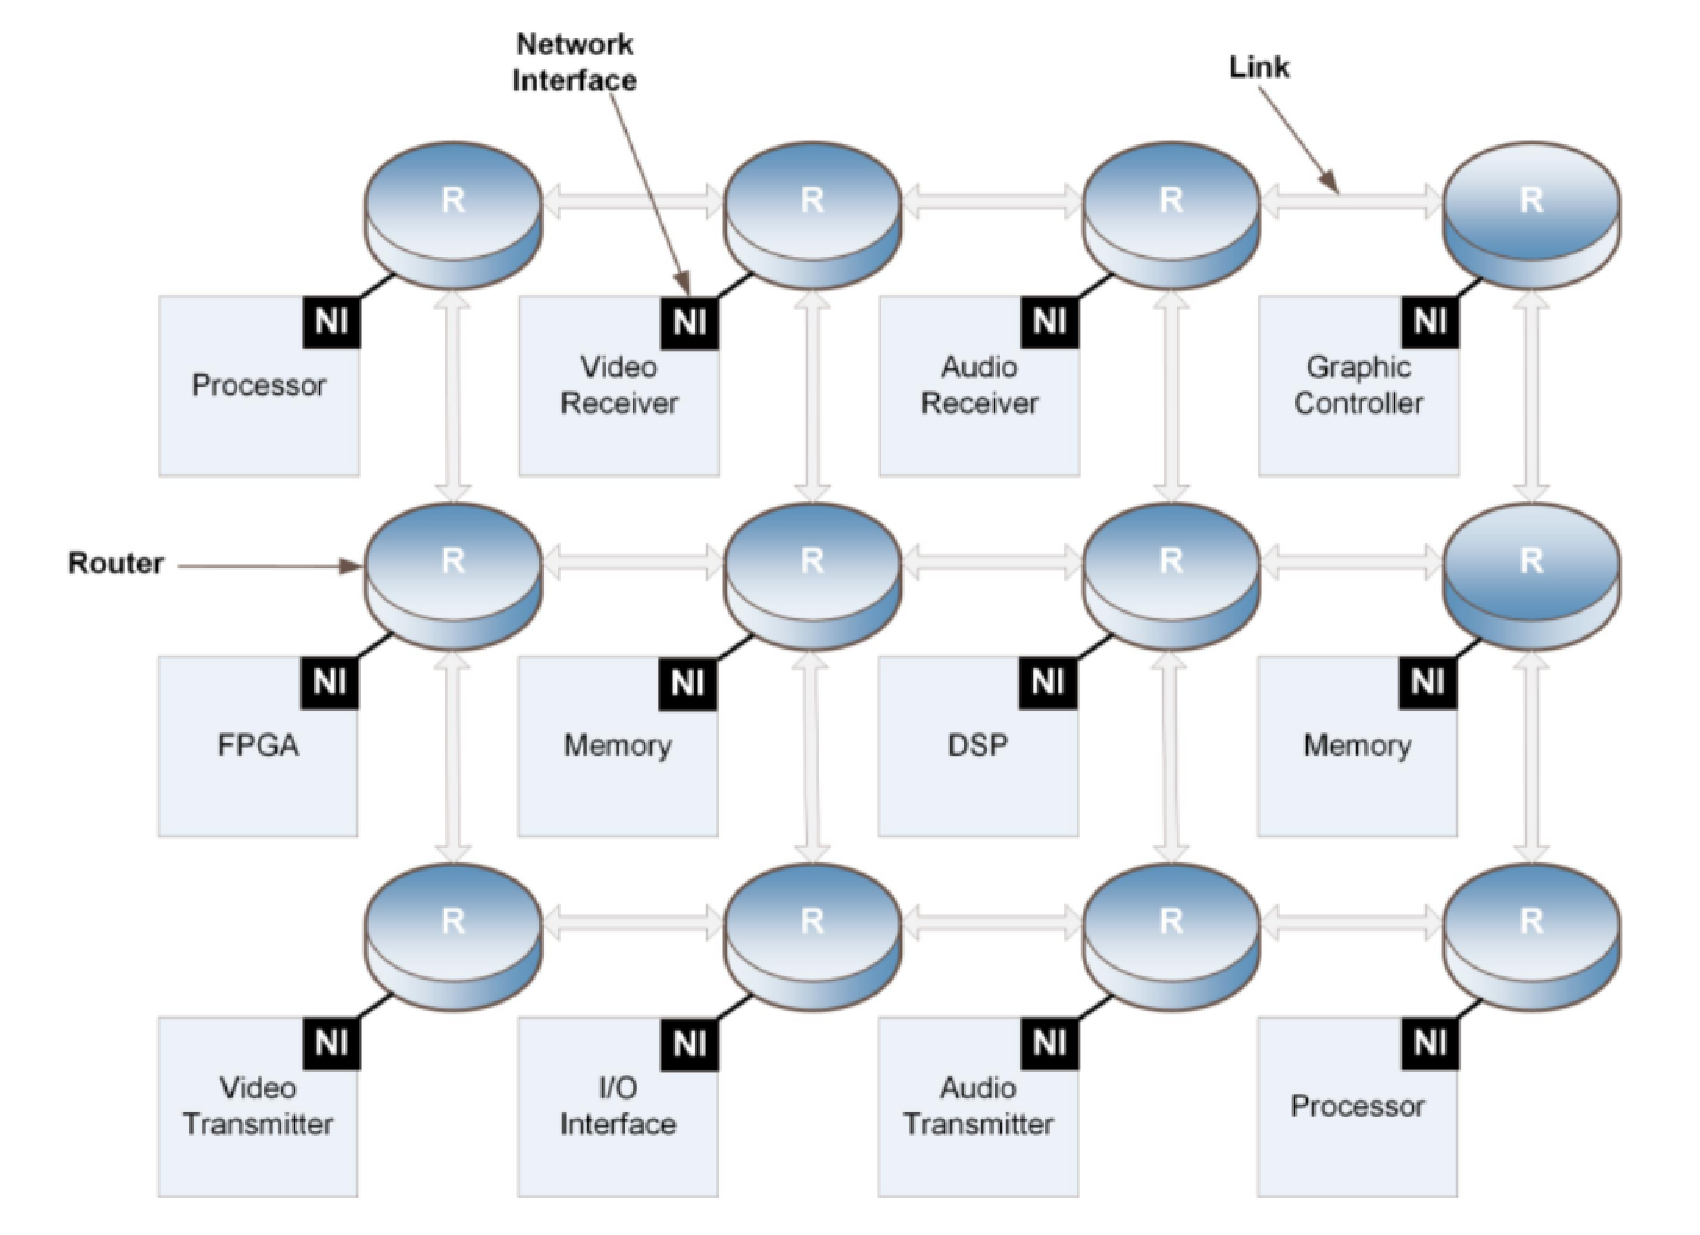
\includegraphics[width=7cm]{NoC}
\caption{NoC system}
    \label{fig:NoC}
\end{figure}

Routers in NoC play a vital role in establishing communication between the IP cores using different protocols called routing algorithms. The routing algorithm is the most significant part of the router because it is mainly responsible for determining the way of moving the packets inside NoC. Developing and enhancing routing algorithms has a direct effect on NoC performance and efficiency.
\subsection{NoC Component}
NoC consists of three main components i.e., routers, links and Network Interfaces(NIs). The data is transmitted from router to router through bidirectional links and each router in NoC is connected to one IP core via the network interface.
\subsubsection{Router}
The router is the most important component in any network and represents the backbone of communication in NoC. Routers in the center nodes in NoC have five ports: East, West, North, South and a Local. The first four ports (East, West, North and South) are connected to the adjacent routers and the Local port is connected to the IP core as shown in Fig.2. The main role of the router in NoC is to receive packets and determine the direction that each packet should take towards the destination. This is determined by using routing protocols that are already implemented inside the router. [1]
\begin{figure}[h]
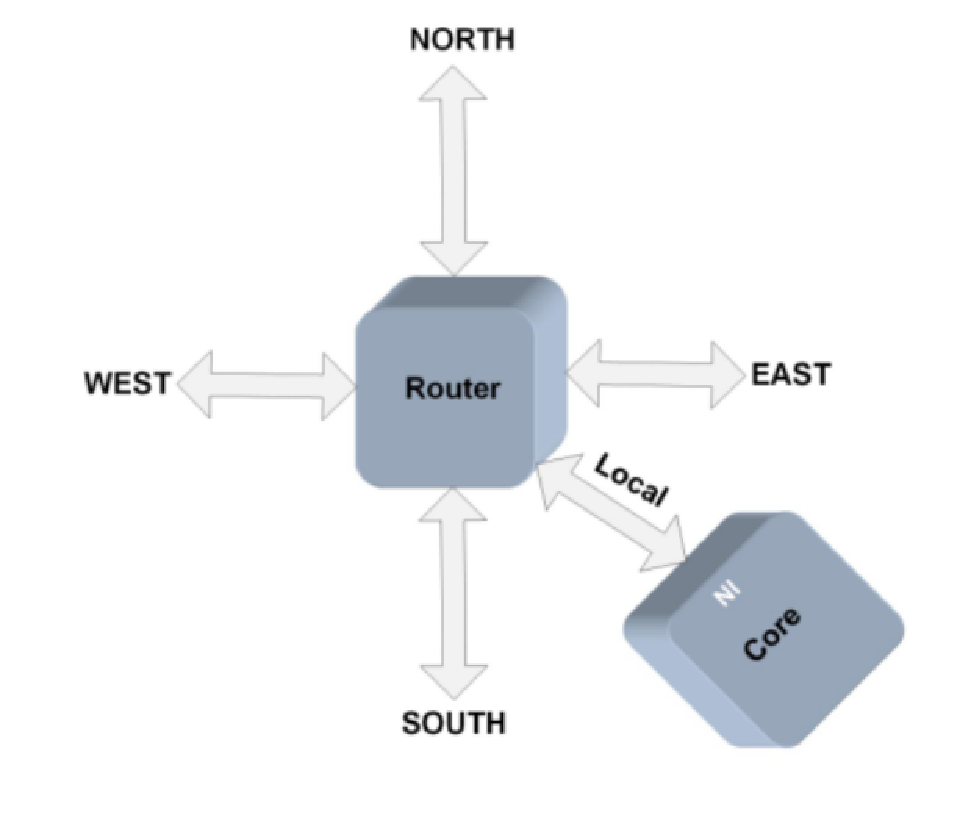
\includegraphics[width=7cm]{router}
\caption{Router}
    \label{fig:router}
\end{figure}

\subsubsection{Links}
The routers in NoC are connected to each other through channels called links. The links also connect each router to one local IP core as shown in Fig.1. The links represent the main way to transmit the packets from router to router or from routers to IP cores. In NoC, the links are bidirectional which provide full-duplex communication between the connected nodes. [1]
\subsubsection{Network Interface}
The network interface is the part of NoC that provides the connection between the routers and IP cores. This interface coordinates the data moving between routers and IP cores in NoC via a full-duplex communication link. When the IP core transmits the data to the network, the data will be first received in the network interface, which packetizes the data and adds destination information to the packets. After that, the routers will read the packet information to route it to the right direction based on the routing algorithm policy in the router. [1]
\subsection{Network Topology}
Network topology is the connecting and arranging of a number of nodes and links in the network. In NoC, several factors, i.e., performance, scalability, power consumption, design complexity, etc., rely on the topology. Moreover, network topology helps to determine the number of nodes inside NoC and decides the length of the links between the nodes. The topology in NoC can be classified into two main categories, i.e., direct and indirect topology. In the direct topology, each router is connected directly to its neighbour routers and to its local IP core. In indirect topology, however, not all routers are connected to the IP cores because some of these routers are used only to propagate the packets inside the network. Also, in indirect topology, the number of routers is larger than the IP cores. In contrast, the number of routers and cores in the direct topology are the same. Examples of the direct topology are mesh, torus, and ring along with fat-tree network topology represents one of the most common examples of indirect topology.

We are going to introduce two of most popular examples of network topology, mesh and torus.
\subsubsection{Mesh}
Mesh topology is the most widely used and simplest direct topology in NoC which consists of $R\times C$ nodes, where R is the number of rows and C is the number of columns in the network. Each router in the nodes is connected to its IP core as shown in Fig.3. Each node in this topology is represented by one IP core and one router. Furthermore, in this topology, the number of cores and the numbers of routers are the same. Fig.3 also shows that the intermediate nodes are connected to four neighbouring nodes, the nodes on the edges are connected to three nodes, and the corner nodes are connected to only two neighbouring nodes. The advantages of mesh topology are that it is easy to implement in NoC since it assumes the same length between the nodes. Because of these advantage in mesh topology, we have applied and tested the proposed routing algorithm in 2D mesh NoC. [1]
\begin{figure}[h]
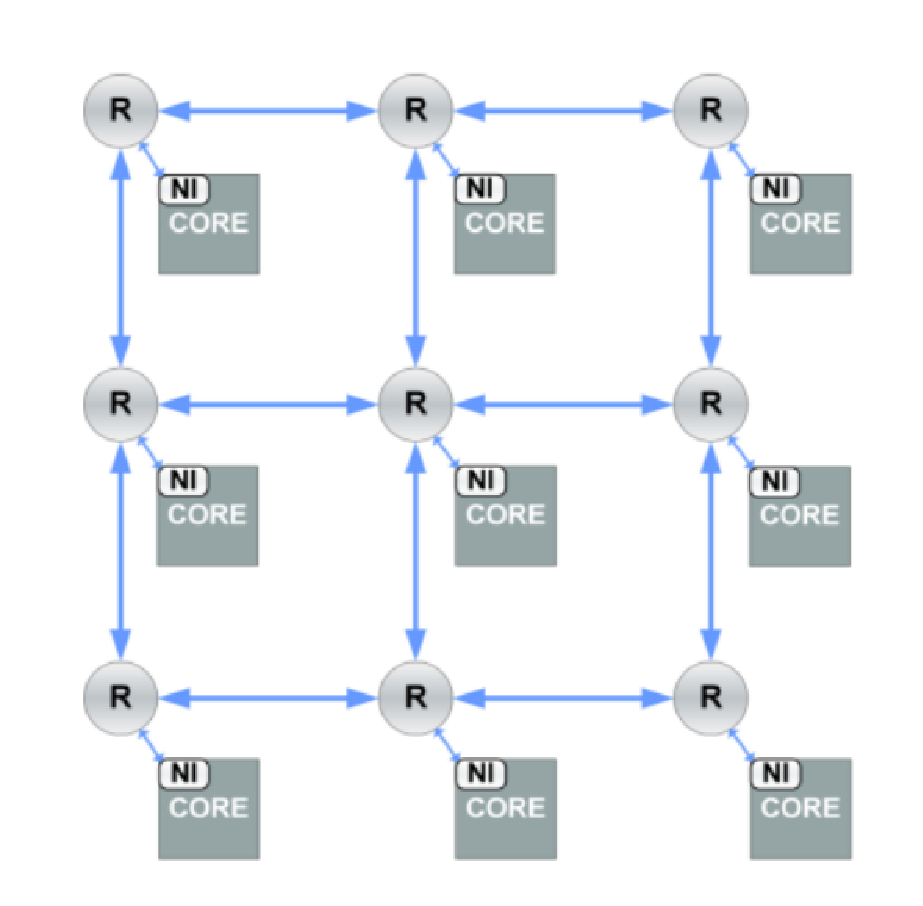
\includegraphics[width=7cm]{mesh}
\caption{Mesh Topology}
    \label{fig:mesh}
\end{figure}
\subsubsection{Torus}
Torus topology is also a type of direct network topology and is similar to mesh topology. However, Torus topology is more complex than mesh topology in terms of implementation because it uses wrap-around links to connect the routers at the edges with the other routers at the opposite edges as shown in Fig.4. The main
disadvantage in Torus topology is that the wrap-around links can result in increase packet propagation delay. In addition, the repeaters which are required through the long links increase the area needed in the network architecture. [1]
\begin{figure}[h]
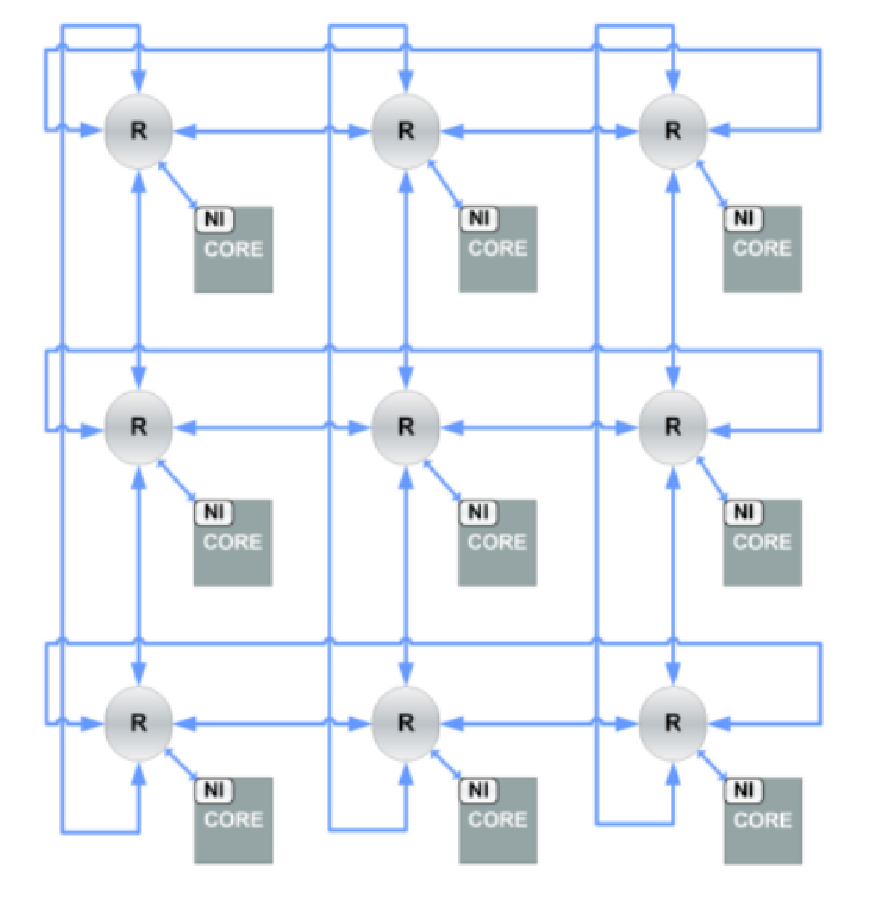
\includegraphics[width=7cm]{torus}
\caption{Torus Topology}
    \label{fig:torus}
\end{figure}

\subsection{Routing Algorithm}
Routing algorithms determine the paths that a packet should take during its journey from the source to the destination. In NoC, the routing algorithms have an essential role to decide the approach for moving the packets between the nodes inside the network. Also, routing algorithms have a direct effect on NoC��s performance, throughput and latency. There are several challenges that may appear with routing algorithms such as deadlock, livelock and starvation. A deadlock is a situation that arises when all the packets routed in the network must wait for each other to release specific channels in a cyclic manner. Consequently, none of the packets can move further and will be kept in a deadlock situation. The problem of livelock occurs when all the packets are moving around the destination but cannot reach it. A starvation problem can happen when certain priorities are assigned to particular packets in NoC. High-priority packets can reach the destination and reserve the resources, making them unreachable by low-priority packets in the network. In the past two decades, many routing algorithms have been proposed to avoid these challenges and improve the performance as well as develop the scalability in NoC. [1]

\section{Related Works}
\label{sec:related works}
We are going to introduce some traditional routing algorithm. Before introducing some traditional algorithm, we are going to claim some definition. The horizontal distance between two nodes can be defined by subtracting X-coordinates of the nodes. Also, the difference between two node��s Y coordinates represents the vertical distance. And $\triangle X$ denotes the horizontal distance between the current node and the destination node. $\triangle Y$ denotes the vertical distance between the current node and the destination node. N denotes the North direction. S denotes the South direction. W denotes the West direction. E denotes the East direction. C denotes the direction pointing to the current IP core.
\subsection{XY routing algorithm}
XY routing algorithm is the simplest method to determine the path from source router to destination router. It relies on the location of source router and destination router. The path will go first in x direction until $\triangle X=0$. Then go in y direction until getting to the destination router. The algorithm is implemented by routers. When a packet is transferred to a router, the router will choose next router as below:
\begin{equation}
next(\triangle X, \triangle Y)=\left\{
\begin{array}{lcl}
C,   &\triangle X=0 \quad and \quad \triangle Y=0\\
E,   &\triangle X>0\\
W,   &\triangle X<0\\
N,   &\triangle X=0 \quad and \quad \triangle Y>0\\
S,   &\triangle X=0 \quad and \quad \triangle Y<0
\end{array}
\right.
\end{equation}
\subsection{MAXY routing algorithm}
MAXY routing algorithm is also a traditional and popular method to determine the path from source router to destination router. It relies on the location of source router and destination router. That the path will go in x direction or y direction will depend on $\triangle X$ and $\triangle Y$. If $\triangle X > \triangle Y$, then go first in x direction. Else, go first in y direction. The algorithm is implemented by routers. When a packet is transferred to a router, the router will choose next router as below:
\begin{equation}
next(\triangle X, \triangle Y)=\left\{
\begin{array}{lcl}
C,   &\triangle X=0 \quad and \quad \triangle Y=0\\
E,   &\triangle X>0 \quad and \quad \triangle X>\triangle Y\\
W,   &\triangle X<0 \quad and \quad \triangle X>\triangle Y\\
N,   &\triangle Y>0 \quad and \quad \triangle X<\triangle Y\\
S,   &\triangle Y<0 \quad and \quad \triangle X<\triangle Y
\end{array}
\right.
\end{equation}
\subsection{FD routing algorithm}
FD routing algorithm relies on the location of the destination node according to the source node as well as it considers the network condition during routing a packet. The FD checks the horizontal and vertical distances between the source and destination nodes and routes the packet horizontally when the horizontal distance is greater than the vertical distance and vice versa. If the horizontal and vertical distances between the source and destination node are the same, FD will route the packet horizontally or vertically based on the network condition in the neighbouring nodes of the source node. This routing algorithm is more complex than XY and MAXY routing algorithm. So the table of routing case in FD routing algorithm shown as in Fig.5 will clearly show how FD routing algorithm works. [1]
\begin{figure}[h]
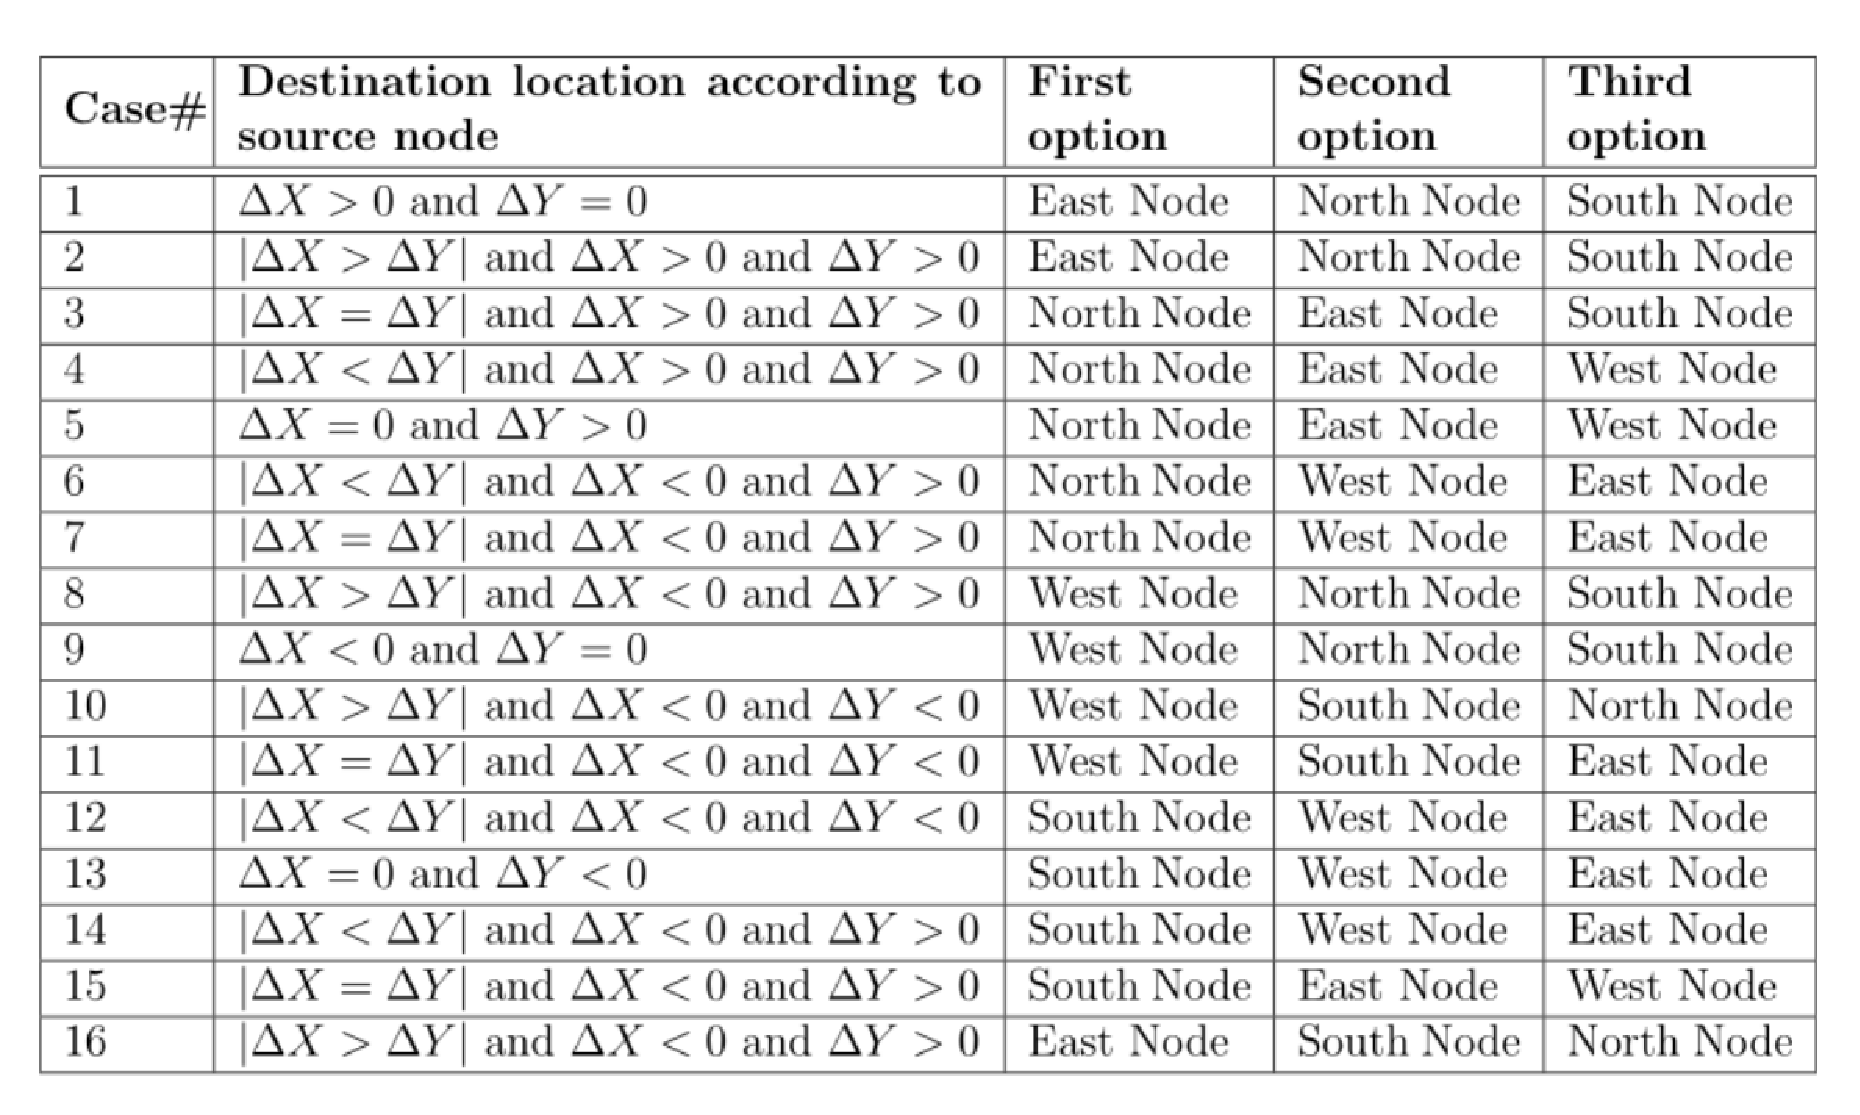
\includegraphics[width=9cm]{FD}
\caption{Routing Cases in FD Routing Algorithm}
    \label{fig:FD}
\end{figure}

\section{Motivation}
\label{sec:motivation}
In NoC, the routing algorithms have an essential role to decide the approach for moving the packets between the nodes inside the network. Also, routing algorithms have a direct effect on NoC��s performance, throughput and latency. However, there are several challenges that may appear with routing algorithms such as deadlock, livelock and starvation. Therefore, we are interested to design some new routing algorithm to improve NoC's performance.

After we explored some traditional routing algorithm, we found that there is few routing algorithm choosing the path to transfer the packets referring to the crowdedness of the whole network. But the crowdedness of network will directly influence the efficiency of NoC. So our group are going to design some routing algorithms which will take the crowdedness of the whole network into consideration.
\section{Problem Formulation}
\label{sec:problem formulation}
Problem Description:

We are going to choose a mesh network topology to explore new routing algorithms. There are several packets going to be routed from different source to different destination. The source router and destination router will be selected randomly. We have to design a routing algorithm to determine the paths for every packet and try to decrease the overall latency.

When a router receives a packet, the router can know its own location, the source router location of the packet, the destination router location of the packet and the condition of whole network. If the router is the destination router, then transfer the packet to the IP core. If not, then the router should choose a direction among North, South, West and East to transfer the packet to next router.

Every router has a buffer to transmit packets. If the buffer has no enough free space, the path passing this router will be blocked temporarily. That is, there is a space limit for routers to transmit packets at the same time. If we want to decrease the overall latency, we need to avoid the situation that the packets are blocked as far as possible.

\section{Proposed Methods}
\label{sec:proposed_methods}
We have proposed two methods about new routing algorithm. Our new routing algorithms rely on the location of source router and destination router and the crowdedness condition of the whole network. Then let's introduce our new routing algorithm in details. At first, we are going to claim some definition. $C(r)$ denotes the crowdedness of the router. In NoC, packets are divided into small units called flit to be transferred. So we define that the number of flits in the router buffer represents the crowdedness of the router. Besides, $C(N)$ denotes the crowdedness of North router. $C(S)$ denotes the crowdedness of South router. $C(W)$ denotes the crowdedness of West router. $C(E)$ denotes the crowdedness of East router.
\subsection{First Method}
First method will take the location as the first factor and the crowdedness as the first factor. At first step, we need to decide the direction on x-axis and y-axis separately according to the destination compared with current point. At second step, according to the crowdedness, we will finally decide to choose x direction or y direction. The specific formula is shown as below:
\begin{equation}
next()=\left\{
\begin{array}{lcl}
C,   &\triangle X=0 \quad and \quad \triangle Y=0\\
arcmin_{r\in \{E,N\}}{C(r)},   &\triangle X>0 \quad and \quad \triangle Y>0\\
arcmin_{r\in \{E,S\}}{C(r)},   &\triangle X>0 \quad and \quad \triangle Y<0\\
arcmin_{r\in \{W,N\}}{C(r)},   &\triangle X<=0 \quad and \quad \triangle Y>0\\
arcmin_{r\in \{W,S\}}{C(r)},   &\triangle X<=0 \quad and \quad \triangle Y<0
\end{array}
\right.
\end{equation}
\subsection{Second Method}
Second method will take the crowdedness as the first factor. Because every router can know the condition of whole network, every router can find the most uncrowded path from the current router to the destination router.
\begin{equation}
path=arcmin_P\sum_{r\in P}C(r)
\end{equation}
Then choose the first router of the path as the next router.

\section{Experiment}
\label{sec:experiment}
We choose NIRGAM as the simulator in our experiment. So we first learn something about NIRGAM.

NIRGAM is a systemC based discrete event, cycle accurate simulator for research in Network on Chip(NoC). It provides substantial support to experiment with NoC design in terms of routing algorithms and applications on various topologies. The architecture of NIRGAM is shown in Fig.6. [2]
\begin{figure}[h]
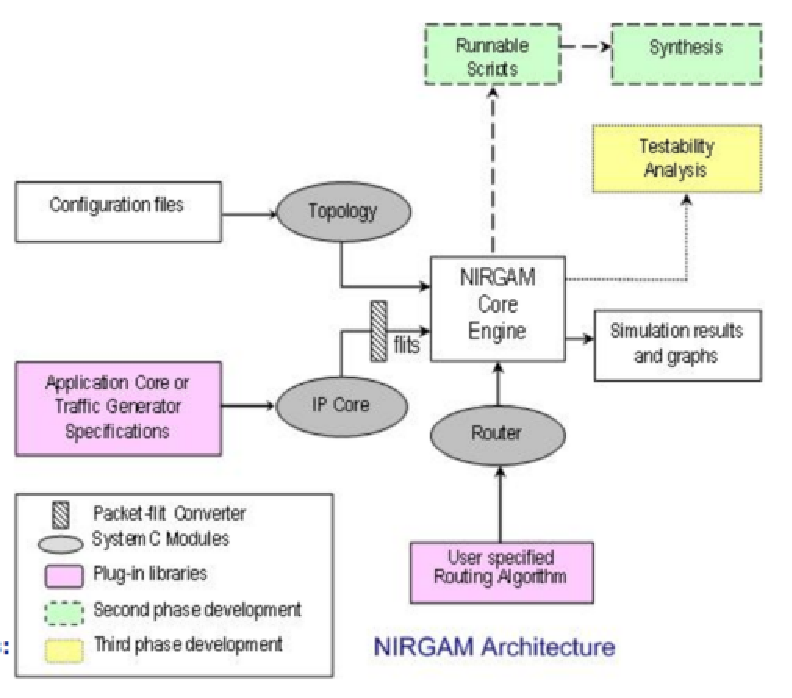
\includegraphics[width=7cm]{NIRGAM}
\caption{the architecture of NIRGAM}
    \label{fig:NIRGAM}
\end{figure}
\subsection{Experiment environment}
Because NIRGAM is based on systemC, we need to download systemC first. Then download the NIRGAM. The OS is Linux. And we choose $5\times 5$ mesh network topology. As for test case, there are five routers randomly selected to play a role as Constant bit rate (CBR) traffic generator. These five routers not only generate the packet, but also receive the packets. And the other routers receive the packets. Besides the destinations of every packet are also random.
\subsection{Add new routers}
The complexity of a router can vary depending upon its intelligence and route logic. You may wish to hack Controller and InputChannel modules to implement any routing algorithm. However a routing algorithm which is a function of source and destination address can be easily implemented as a class derived from class router. Next we will explain steps to add such a router. As an example let us consider that we need to add a routing algorithm identified by name "R" and library name "myrouter.so".

1. Run "make clean".

2. Create header file myrouter.h in \$NIRGAM/router/src. A template file is included in source code for your reference.

3. Create implementation file myrouter.cpp in \$NIRGAM/router/src. A template file is included in source code for your reference.

4. Edit calc\_next() function in myrouter.cpp to insert your route logic.

5. Edit \$NIRGAM/config/constantss.h to include name of your routing algorithm (R).

6. Edit \$NIRGAM/core/Controller.cpp to enable the controller to attach router library.

7. Edit Makefile to include name of source file in ROUTER\_SRCS.

8. Run make.
\subsection{Running simulation}
After make, then run the executable file 'nirgam' to run simulation. And we can edit nirgam.config and application.config to adjust some parameter of simulation. nirgam.config is the main configuration file that contains parameters specific to NoC design and simulation. And application.config file lets you specify application mapping. It accepts input as pairs of tileID and name of application library to be attached to the tile. The applications that can be attached are stored in \$NIRGAM/application/lib. And the result of simulation will be stored in \$NIRGAM/result.
\section{Conclusion}
\label{sec:conclusion}
The result of experiments is shown in Fig.7.
\begin{figure}[h]
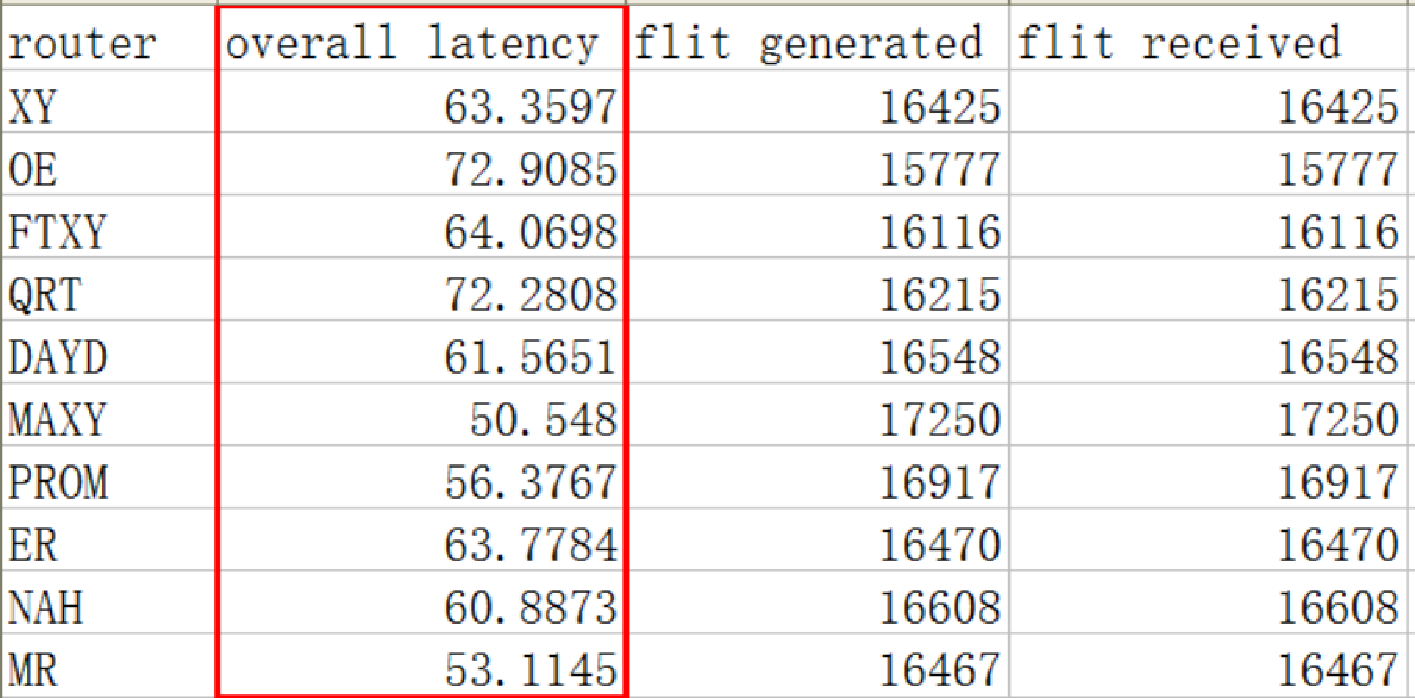
\includegraphics[width=7cm]{result}
\caption{the result of experiment}
    \label{fig:result}
\end{figure}

We run the simulation with using 10 kinds of routing algorithm. Two of these routing algorithm are out new routing algorithms. They are identified by name "NAH" and "MR". According to the result, we find that our new routing algorithms have a better performance than most of traditional routing algorithm. What's more, the time complexity of routing algorithm will also increase the overall latency to transfer the packets. We need find a balance between the complexity and the efficiency of routing algorithm.

\section{reference}

[1]:Design and Evaluation of Force-Directed (FD) Routing Algorithm in 2D Mesh Network on Chip, Kasem Shwiegi.

[2]:NIRGAM manual

\end{document}
% End of v2-acmtog-sample.tex (March 2012) - Gerry Murray, ACM
